\documentclass[12pt]{scrartcl}
\usepackage[utf8]{inputenc}
\usepackage{booktabs}
\usepackage{xspace}
\usepackage{caption}
\usepackage{subcaption}
\usepackage{txfonts}
\usepackage{notoccite}
\usepackage{hyperref}
\usepackage[spanish,es-tabla]{babel}
\renewcommand{\sectfont}{\rmfamily \bfseries}


\title{Aplicación de computación en paralelo para evaluación de SVM con validación cruzada}
\author{Ignacio Suárez Andrés}
\date{20 de abril de 2015}
\usepackage{Sweave}
\begin{document}
\Sconcordance{concordance:informesvm.tex:informesvm.Rnw:%
1 16 1 1 0 87 1 1 7 17 0 1 3 1 7 17 0 1 3 1 7 17 0 1 9 17 0 1 3 12 1}

\maketitle
\section{Introducción}
Cuando se trabaja con grandes volúmenes de datos o modelos complejos para problemas de clasificación, es común realizar la evaluación y validación de los ajustes con una partición simple de los datos en subconjuntos de entrenamiento y test, en lugar de técnicas más avanzadas como la validación cruzada, debido al elevado coste computacional que ésta supone.\par
Como propuesta frente a este problema, se ha realizado un ejercicio de implementación de la validación cruzada en R \cite{Rcita} para entrenamiento y evaluación de máquinas de vectores soporte (SVM) empleadas como clasificadores, que puede servir de base para ser aplicado a problemas más avanzados.\par
\section{Máquinas de Vectores Soporte (SVM)}
Las máquinas de vectores soporte (en adelante SVM, por sus siglas en inglés) son un tipo de algoritmo de \textit{machine learning} supervisado, empleado principalmente para clasificación aunque tiene también aplicaciones en regresión \cite{islr}.\par
La idea fundamental de las SVM es la búsqueda de un hiperplano que marque una frontera lineal entre las clases de datos. Un hiperplano es un subespacio plano de dimensión $D-1$, donde $D$ es la dimensión de los datos. Para que la elección del hiperplano sea única, se busca maximizar la distancia respecto de los puntos a ambos lados de la frontera, como se muestra en la figura \ref{fig:svmlineal}. Lo que hace especial a este algoritmo es que el hiperplano queda delimitado únicamente en función de un conjunto de puntos cercanos a la frontera, apropiadamente denominados vectores soporte.\par

\begin{figure}[h]
\centering
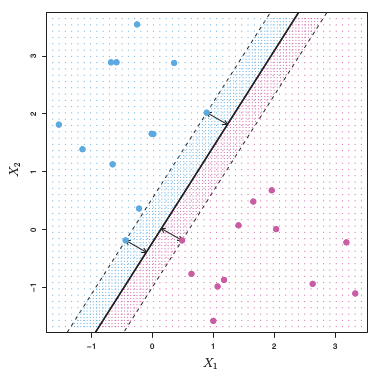
\includegraphics [width=8 cm]{svmlinear}
\caption{Hiperplano de máxima distancia entre dos clases de datos linealmente separables.}
\label{fig:svmlineal}
\end{figure}

Un clasificador lineal de vectores soporte, sin entrar en detalles de su computación, se puede representar como
\begin{equation}
f(x) = \beta_0 + \sum_{i \in \mathcal{S}} \alpha_i \langle x,x_i \rangle
\end{equation}
donde $\langle x,x_i \rangle$ es el producto interno de los vectores $x$ y $x_i$, $\alpha_i$ y $\beta_0$ dependen de los productos internos de todos los pares de vectores del conjunto de entrenamiento, y $\mathcal{S}$ indica el conjunto de vectores soporte, y que $\alpha_i$ es nulo para vectores del conjunto de entrenamiento que no sean soporte.\par
Para datos no linealmente separables, este concepto se generaliza sustituyendo el producto interno $\langle x,x_i \rangle$ por un kernel $K(x,x_i)$, siendo este caso cuando se habla propiamente de máquinas de vector soporte. En este trabajo se utiliza el kernel de tipo polinómico, que tiene la siguiente forma:
\begin{equation}
K(x,x_i)=\left(1+\langle x,x_i \rangle \right)^d
\end{equation}
siendo $d$ el grado del polinomio. Esta construcción permite llevar el problema a un espacio de dimensión superior donde los datos sí sean linealmente separables.\par

Cuando los datos no son totalmente separables, sino que existe una cierta mezcla cerca de la frontera, se puede introducir en el entrenamiento del SVM un parámetro llamado coste, que indica el entorno de la frontera en el que se admiten puntos mal clasificados. La figura \ref{fig:coste} proporciona una explicación visual de los efectos de este parámetro.\par

Se ha utilizado la implementación de SVM contenida en el paquete \href{http://cran.r-project.org/web/packages/e1071/index.html}{\texttt{e1071}} de R.

\begin{figure}[h]
\centering
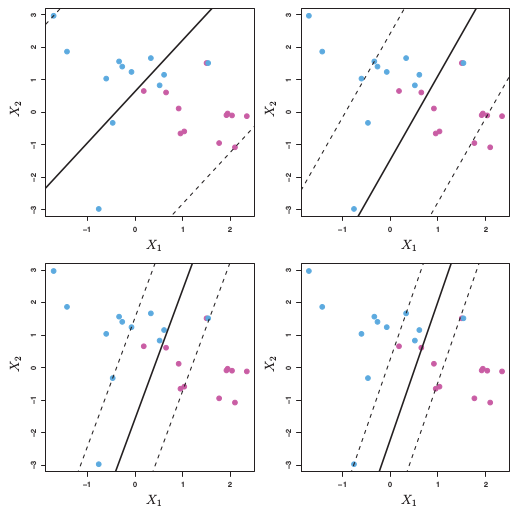
\includegraphics [width=12 cm]{svmcost}
\caption{Efectos de pasar de un parámetro de coste alto (arriba a la izquierda) hacia uno bajo (abajo a la derecha). Esto tiene la consecuencia de pasar de muchos vectores soporte (alto potencial de sesgo, baja varianza) a pocos (bajo sesgo, mucha varianza).}
\label{fig:coste}
\end{figure}

\clearpage
\section{Validación cruzada}
Para evaluar un modelo de clasificación (o de regresión) es común utilizar un conjunto de datos de entrenamiento y uno de test. Uno de los métodos más eficientes es la validación cruzada con 10 subconjuntos (ten-fold cross-validation), preferiblemente respetando las proporciones entre clases en cada uno \cite{khv}.\par
El método consiste en dividir el conjunto total de datos en 10 subconjuntos. A continuación, se entrena y evalúa repetidamente el modelo, tomando en cada iteración uno de los 10 subconjuntos para test y el resto para entrenamiento.\par
De este modo, se puede evaluar si los parámetros o la precisión del modelo son robustos frente a pequeñas variaciones en el conjunto de datos de entrenamiento. Dado que las iteraciones son independientes entre sí, existe la oportunidad de paralelizar este proceso fácilmente.\par
La partición de los datos se ha realizado con funciones del paquete \href{http://cran.r-project.org/web/packages/cvTools/index.html}{\texttt{cvTools}} de R.\par


\section{Paralelización en R}
Los paquetes \href{http://cran.r-project.org/web/packages/doParallel/index.html}{\texttt{doParallel}} y \href{http://cran.r-project.org/web/packages/foreach/index.html}{\texttt{foreach}} de R permiten la ejecución de bucles iterativos de tipo `for' en paralelo.\par
El primer paso consiste en registrar las unidades de procesamiento que se emplearán, ya sea un determinado número de núcleos o un cluster de procesadores. Esto permite la paralelización de un bucle `foreach', sustituto del `for', siempre que se especifique la opción `\%dopar\%'.\par
La forma de recoger la salida de un bucle `foreach' es bastante peculiar, ya que depende de que se evalúe una expresión en cada iteración del bucle, cuyo valor es recogido en un objeto de tipo lista. Por otra parte, existe cierta flexibilidad para controlar la estructura de la lista, estando permitido que los datos se agrupen formando una matriz contenida en la lista. Es posible incluso definir funciones personalizadas que den lugar a estructuras más complejas, como se realizó en este trabajo, extrayéndose una lista que contiene a su vez dos listas con diez matrices cada una.\par

\section{Aplicación}
Para aplicar todos los conceptos anteriores se ha generado un conjunto de 2000 parejas de números aleatorios, divididas en dos clases mediante una función arbitraria con un término aleatorio que introduce una ligera mezcla en la frontera entre clases. La figura \ref{fig:puntos} muestra estos puntos.\par

\begin{figure}[]
\centering
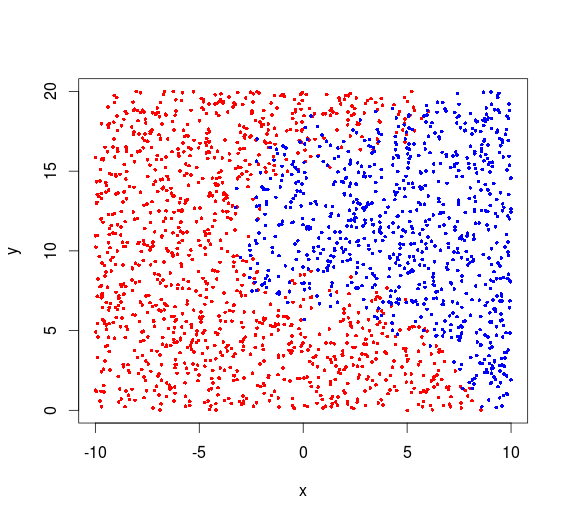
\includegraphics [width=10 cm]{points}
\caption{Conjunto de puntos a clasificar.}
\label{fig:puntos}
\end{figure}

Tras particionar los datos para la validación cruzada, se itera de modo paralelo sobre las posibles elecciones de conjuntos de entrenamiento y de test. Para cada una, se entrena y evalúa la SVM para el siguiente rango de valores de los parámetros del kernel polinómico:
\begin{itemize}
\item Coste: 0.01, 0.1, 1, 10, 100, 1000.
\item Grado: 1, 2, 3, 4, 5, 6.
\end{itemize}

El método escogido para evaluar el ajuste de cada SVM es el área bajo la curva ROC (AUC, \textit{area under curve}). Una curva ROC, como la de la figura \ref{fig:roc}, indica el comportamiento del clasificador en función del valor de corte que determina su sensibilidad. La integral entre 0 y 1 de esta curva, es decir, el área bajo ella, toma un valor de 1 en el caso de clasificación óptima (ó 0, si discriminase perfectamente pero asignase las clases al revés) y de 0.5 para un clasificador aleatorio, que sería el peor escenario.\par

\begin{figure}[hb]
\centering
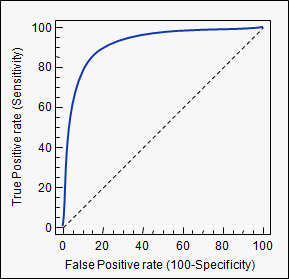
\includegraphics [width=5.45 cm]{roc}
\caption{Curva ROC: Tasa de verdaderos positivos frente a tasa de falsos positivos, en función del parámetro de corte empleado en la clasificación.}
\label{fig:roc}
\end{figure}


El AUC es un buen indicador de sobreajuste, que se manifiesta como un valor notablemente mejor para los datos de entrenamiento que para los de test. La robustez del modelo se puede evaluar además viendo si estos valores fluctúan ampliamente al variar la partición de los datos escogida para el entrenamiento.\par





\section{Resultados}
Se ha entrenado y evaluado la SVM mediante validación cruzada con 10 iteraciones ejecutada en paralelo, para 6 valores de los parámetros de coste (tolerancia) de puntos mal clasificados y grado del kernel polinómico. Se ha tomado la media de los valores AUC obtenidos en cada iteración de entrenamiento, así como su desviación estándar para comprobar si existe sensibilidad a variaciones en los datos. Se proporcionan los valores de AUC para los datos de entrenamiento y de test, para determinar la posible existencia de sobreajuste. Estos resultados están contenidos en las tablas \ref{table:train}, \ref{table:test}, \ref{table:sdtrain} y \ref{table:sdtest}.\par
Se obtienen los mejores resultados para kernel polinómico de grado impar, con independencia del coste. No se observa tendencia al sobreajuste ni sensibilidad a las variaciones en los datos de entrenamiento.\par
La ejecución de los entrenamientos y evaluaciones de las SVM se ha realizado en paralelo sobre 4 núcleos entre los que se reparten las iteraciones sobre diferentes subconjuntos de la validación cruzada. Con esto, el tiempo de ejecución de esta parte del código se redujo a un 56\% del tiempo requerido para la computación en serie.\par
% latex table generated in R 3.1.3 by xtable 1.7-4 package
% Mon Apr 20 13:14:49 2015
\begin{table}[ht]
\centering
\begin{tabular}{rrrrrrr}
  \hline
 & 1 & 2 & 3 & 4 & 5 & 6 \\ 
  \hline
0.01 & 0.9245 & 0.6904 & 0.9037 & 0.7150 & 0.9024 & 0.6780 \\ 
  0.1 & 0.9250 & 0.6944 & 0.9227 & 0.7166 & 0.9053 & 0.6931 \\ 
  1 & 0.9248 & 0.6985 & 0.9230 & 0.7268 & 0.9219 & 0.7113 \\ 
  10 & 0.9248 & 0.6986 & 0.9226 & 0.7266 & 0.9226 & 0.7171 \\ 
  100 & 0.9248 & 0.6986 & 0.9225 & 0.7264 & 0.9211 & 0.7176 \\ 
  1000 & 0.9248 & 0.6986 & 0.9228 & 0.7279 & 0.9183 & 0.7177 \\ 
   \hline
\end{tabular}
\caption{Valores medios de AUC para los subconjuntos de entrenamiento. Las filas indican el parámetro coste, las columnas el grado del polinomio del kernel.} 
\label{table:train}
\end{table}
% latex table generated in R 3.1.3 by xtable 1.7-4 package
% Mon Apr 20 13:14:49 2015
\begin{table}[ht]
\centering
\begin{tabular}{rrrrrrr}
  \hline
 & 1 & 2 & 3 & 4 & 5 & 6 \\ 
  \hline
0.01 & 0.9246 & 0.6916 & 0.9028 & 0.7088 & 0.9025 & 0.6769 \\ 
  0.1 & 0.9246 & 0.6950 & 0.9223 & 0.7070 & 0.9049 & 0.6916 \\ 
  1 & 0.9242 & 0.6987 & 0.9227 & 0.7278 & 0.9205 & 0.7090 \\ 
  10 & 0.9242 & 0.6991 & 0.9221 & 0.7269 & 0.9214 & 0.7176 \\ 
  100 & 0.9241 & 0.6991 & 0.9220 & 0.7268 & 0.9182 & 0.7184 \\ 
  1000 & 0.9241 & 0.6991 & 0.9217 & 0.7289 & 0.9157 & 0.7183 \\ 
   \hline
\end{tabular}
\caption{Valores medios de AUC para los subconjuntos de test. Las filas indican el parámetro coste, las columnas el grado del polinomio del kernel.} 
\label{table:test}
\end{table}
% latex table generated in R 3.1.3 by xtable 1.7-4 package
% Mon Apr 20 13:14:49 2015
\begin{table}[ht]
\centering
\begin{tabular}{rrrrrrr}
  \hline
 & 1 & 2 & 3 & 4 & 5 & 6 \\ 
  \hline
0.01 & 0.0023 & 0.0055 & 0.0022 & 0.0080 & 0.0035 & 0.0139 \\ 
  0.1 & 0.0023 & 0.0069 & 0.0024 & 0.0078 & 0.0025 & 0.0120 \\ 
  1 & 0.0023 & 0.0041 & 0.0022 & 0.0066 & 0.0026 & 0.0189 \\ 
  10 & 0.0023 & 0.0040 & 0.0021 & 0.0058 & 0.0028 & 0.0167 \\ 
  100 & 0.0023 & 0.0040 & 0.0021 & 0.0056 & 0.0024 & 0.0159 \\ 
  1000 & 0.0023 & 0.0040 & 0.0023 & 0.0061 & 0.0039 & 0.0163 \\ 
   \hline
\end{tabular}
\caption{Desviaciones estándar de AUC para los subconjuntos de entrenamiento. Las filas indican el parámetro coste, las columnas el grado del polinomio del kernel.} 
\label{table:sdtrain}
\end{table}% latex table generated in R 3.1.3 by xtable 1.7-4 package
% Mon Apr 20 13:14:49 2015
\begin{table}[ht]
\centering
\begin{tabular}{rrrrrrr}
  \hline
 & 1 & 2 & 3 & 4 & 5 & 6 \\ 
  \hline
0.01 & 0.0207 & 0.0308 & 0.0241 & 0.0287 & 0.0275 & 0.0315 \\ 
  0.1 & 0.0210 & 0.0305 & 0.0213 & 0.0324 & 0.0235 & 0.0338 \\ 
  1 & 0.0216 & 0.0312 & 0.0191 & 0.0362 & 0.0245 & 0.0500 \\ 
  10 & 0.0216 & 0.0309 & 0.0191 & 0.0363 & 0.0209 & 0.0519 \\ 
  100 & 0.0215 & 0.0309 & 0.0191 & 0.0369 & 0.0188 & 0.0511 \\ 
  1000 & 0.0216 & 0.0310 & 0.0190 & 0.0344 & 0.0166 & 0.0530 \\ 
   \hline
\end{tabular}
\caption{Desviaciones estándar de AUC para los subconjuntos de test. Las filas indican el parámetro coste, las columnas el grado del polinomio del kernel.} 
\label{table:sdtest}
\end{table}\clearpage
\section{Conclusiones}
\begin{itemize}
\item Se ha paralelizado un problema de entrenamiento y evaluación de SVM para diferentes parámetros con validación cruzada.
\item Se han extraído correctamente los datos con el formato que impone la paralelización en R, pudiéndose obtener conclusiones como que funcionan mejor los kernel polinómicos de grado impar, no influye el parámetro coste, no se da sobreajuste y no se aprecia sensibilidad frente a fluctuaciones en los datos de entrenamiento.
\item La paralelización ha permitido reducir el tiempo de ejecución de este proceso a un 56\% del tiempo requerido en serie al utilizar 4 núcleos.
\item La idea del ejercicio es aplicable a problemas más complejos o con más datos, especialmente en caso de disponibilidad de grandes números de procesadores o núcleos.
\end{itemize}


\bibliographystyle{unsrt}
\bibliography{mybib.bib}
\end{document}
